%*----------- SLIDE -------------------------------------------------------------
\begin{frame}[t]{O que é docker?} 
    \transdissolve[duration=0.5]
    É uma plataforma \textit{open source} para desenvolver, enviar e rodar aplicativos em um ambiente isolado chamado de \textit{container}.

    A tecnologia foi iniciada em 2013 pela Docker Engine para sistemas Linux, utilizando de conceitos primitivos como \textit{cgroups} e \textit{namespaces} para segregar processos.\cite{redhat}
    
    \begin{figure}
        
\includegraphics[width=.3\textwidth]{homepage-docker-logo}
    \end{figure}
%*----------- notes
    \note[item]{Notes can help you to remember important information. Turn on the notes option.}
\end{frame}
%-
%*----------- SLIDE -------------------------------------------------------------
\begin{frame}[t]{O que são \textit{containers}?} 
    \transdissolve[duration=0.5]
    \begin{columns} 
        \column{.5\textwidth}
            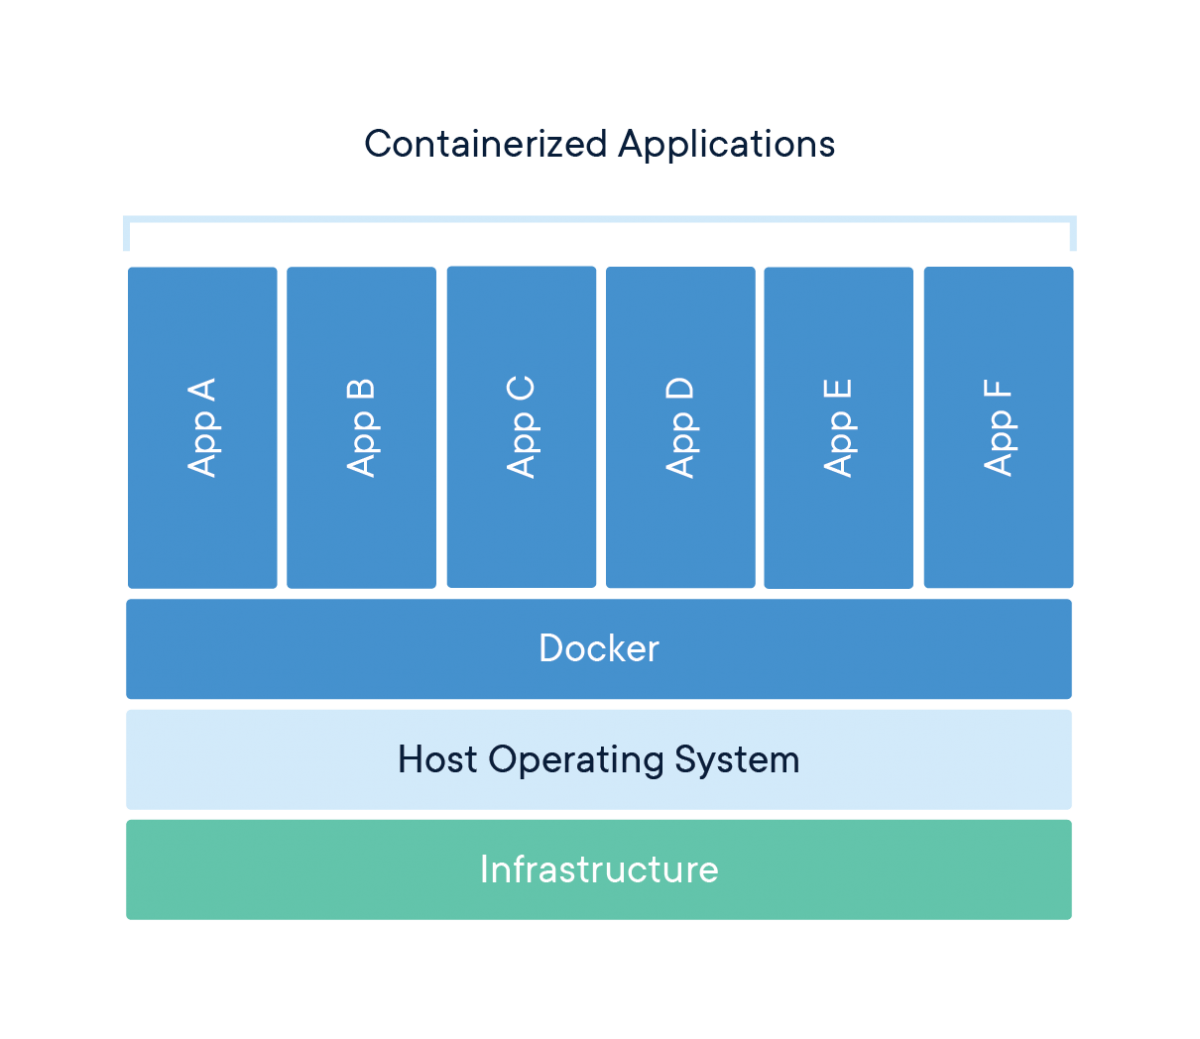
\includegraphics[width=1.1\textwidth]{container-what-is-container.png}
        \column{.5\textwidth}
            \begin{itemize}
                \item \textit{Container} é a unidade padrão do software que empacota o código e suas dependências
                \item É isolado a nível de disco, memória, processamento e rede
                \item É criado a partir de uma Imagem Docker
            \end{itemize}
          
    \end{columns}
%*----------- notes
    \note[item]{Notes can help you to remember important information. Turn on the notes option.}
\end{frame}
%-
%*----------- SLIDE -------------------------------------------------------------
\begin{frame}[t]{Arquitetura} 
    \transdissolve[duration=0.5]

    \begin{figure}
        \centering
        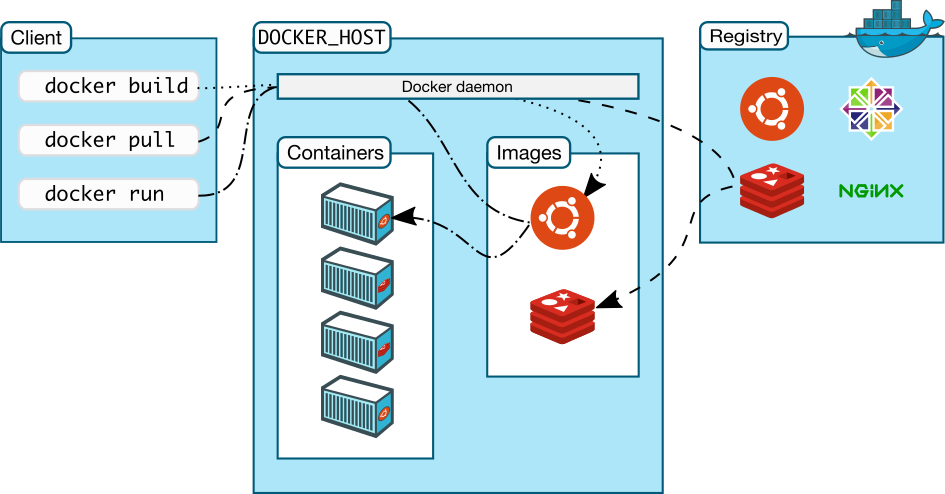
\includegraphics[width=.7\textwidth]{architecture_docker}
        \caption{\cite{docker-overview}}
    \end{figure}
%*----------- notes
    \note[item]{Notes can help you to remember important information. Turn on the notes option.}
\end{frame}
%-